\subsection{Location Sharing}
\label{subsec-locationsharing}

\begin{table}[t]
\begin{tabularx}{\columnwidth}{XXXXX}
\multicolumn{1}{c}{\normalsize{\textbf{Gap}}} &
\multicolumn{2}{c}{\normalsize{\textbf{GPS}}} &
\multicolumn{2}{c}{\normalsize{\textbf{Network}}} \\
\multicolumn{1}{c}{(min)} &
\multicolumn{1}{l}{Hits} &
\multicolumn{1}{l}{\%} &
\multicolumn{1}{l}{Hits} &
\multicolumn{1}{l}{\%} \\
\toprule
5 & \num{4742} & 1.4 & \num{71444} & 10.3 \\
10 & \num{5486} & 1.6 & \num{79877} & 20.5 \\
15 & \num{6064} & 1.8 & \num{85091} & 21.9 \\
20 & \num{6450} & 1.9 & \num{88990} & 22.9 \\
\midrule
\textbf{Total} & \multicolumn{2}{l}{\num{340084}} & \multicolumn{2}{l}{\num{388800}} \\
\end{tabularx}
\caption{\textbf{Coordinate sharing counts.} We discovered few opportunities
to reduce GPS usage through coordinate sharing.}
\label{table-locationsharing}
\end{table}

Location tracking has been the focus of many recent mobile systems research
efforts~\cite{kim:sensys:2010, paek:mobisys:2010, kjaergaard:mobisys:2011}.
Given \PhoneLab{}'s density and stable set of participants, it provides an ideal
proving ground for new location techniques.

One promising idea is to reduce GPS usage through local coordinate sharing.
Before taking a reading, a smartphone will use a local communication protocol
to determine whether a device nearby has recently obtained a GPS reading. If
so, and if that reading is sufficiently recent and accurate, the device may
not have to turn on its GPS at all, reducing latency and saving power. As a
more complex variant, multiple readings from different nearby devices at
different times could be combined to produce a new, more accurate reading.

Previous work~\cite{paek:mobisys:2010} has included the more limited form of GPS
coordinate sharing into their location management system. However, given that
the evaluation was done using five phones traveling in a backpack together,
it is likely that their experiment evaluated nearly the best case for this
approach. Given that \PhoneLab{} provides access to a dense set of
participants, it would seem a good fit for determining whether GPS coordinate
sharing has merit.

\begin{figure*}[t]
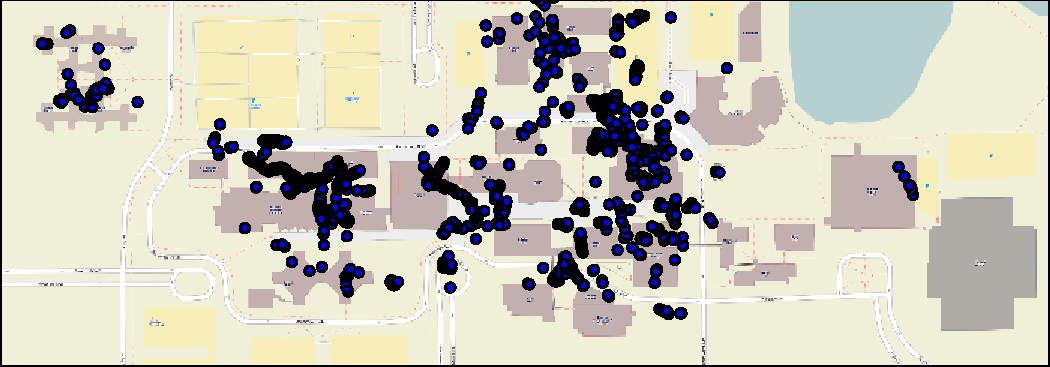
\includegraphics[width=\textwidth]{./figures/location/loc_sharing/map_gps_all.pdf}
\caption{\textbf{Location of GPS sharing opportunities.}}
\label{fig-locationsharing}
\end{figure*}

\subsubsection{Can smartphones share?}

To answer this question we process the data from our usage experiment. In
order for GPS coordinate sharing to take place, several conditions must be
true. First, the two phones must be nearby in time and space. We use the
location updates logged by our experiment to determine this.

Note that we assume that the participant remained at the place where they
acquired the location information for the time necessary to participate in
sharing. While this assumption clearly does not hold in any case, mobility
would not necessarily bias our result in either direction. For every false
positive, a participant that did not remain where they obtained the last
location fix, there may be a corresponding false negative: a participant that
moved and ended up nearby another participant without our knowledge.

The second requirement is that the first phone acquire a location with
sufficient accuracy to satisfy the second device. We use the accuracy
estimation provided by the Android location manager to determine this.

Table~\ref{table-locationsharing} summarizes our negative result: we find few
opportunities for GPS sharing on our testbed. The table is interpreted as
follows: of the \num{3400084} total GPS updates performed during the three
week study, only \num{4742} could have been satisfied with a less that five
minute old coordinate from a nearby device of equal accuracy.

Obviously the effectiveness of collaborative protocols increases as more
phones participate in them, meaning that this result may be interpreted as
indicating that GPS coordinate sharing would require higher densities to be
effective. However, as a point of comparison we present numbers for network
coordinate sharing in Table~\ref{table-locationsharing}. The interpretation
of the data is the same except in this case the phone is using a network,
rather than GPS, provider. Given that the power overhead for obtaining a
network location is likely to be similar to retrieving one from a nearby
phone, this is not necessary a positive result, but it does help put the low
GPS sharing numbers in context.

\subsubsection{Future Experiments}

We expect location management to continue to be an active area of research
and \PhoneLab{} to play a major role. With the ability to change or replace
the Android location service, new approaches to location estimation, sharing,
and tracking can be evaluated without altering installed applications. An
area of future study, however, would be ways of determining whether new
location approaches are experienced as equivalent or better by \PhoneLab{}
participants.

In addition with the rise of new phone-to-phone communication protocols such
as Wifi Direct~\cite{wifi-direct}\footnote{Despite no official support for Wifi
Direct on the Nexus S by the AOSP, we were able to enable this feature and
will distribute it on future platform images. The next generation of
\PhoneLab{} phones should have official AOSP support for this useful
feature.}, we expect \PhoneLab{} to host new research that harnesses the
power of device interaction. We are working on establishing low-overhead
methods for discovering and counting nearby \PhoneLab{} participants in order
to do contact studies and explore participant social networks.
